\section{Gravity waves}
\label{sec:gw}

\TODO{introduce the test, justify its purpose}
\TODO{it might be nice to have some theory on gravity waves (e.g. how theta/w anomalies are created and their positions in space), then compare model results with theory}

\subsection{Specification}
Following \textcite{melvin2010}, the domain is \SI{300}{\kilo\meter} wide and \SI{30}{\kilo\meter} high.  The mountain profile has the same form as equation~\ref{eqn:resting:mountain} but with a lower maximum height of $\surface_0 = \SI{250}{\meter}$.  As in the resting atmosphere test, $a = \SI{5}{\kilo\meter}$ is the mountain half-width and $\lambda = \SI{4}{\kilo\meter}$ is the wavelength.  On the optimised SLEVE grid, $s_1 = \SI{5}{\kilo\meter}$ is the large scale height, $s_2 = \SI{2}{\kilo\meter}$ is the small scale height and the optimal exponent value $n = 1.35$ as in the previous test\TODOsidenote{where did these SLEVE parameters come from?}.

The initial thermodynamic conditions have a surface temperature of $\theta_0 = \SI{288}{\kelvin}$ and constant stability with $N = \SI{0.01}{\per\second}$ everywhere.  A constant horizontal wind $u = \SI{10}{\meter\per\second}$ is prescribed at the inlet boundary.

\subsection{Discretisation}
The test uses the discretisation of the Euler equations described in section~\ref{sec:method:discretisation}.  The domain is discretised on a grid having $600 \times 100$ cells such that $\Delta x = \SI{0.5}{\kilo\meter}$ and $\Delta z = \SI{300}{\meter}$.  Sponge layers are added to the upper \SI{10}{\kilo\meter} and leftmost \SI{10}{\kilo\meter} at the inlet boundary to damp the reflection of waves.
The term $\mu \rho \vect{u}$ is subtracted from the momentum equation (equation~\ref{eqn:method:momentum}) where the damping function $\mu$ is adapted from \textcite{melvin2010} such that
\begin{align}
	\mu(x, z) &= \mu_\mathrm{upper} + \mu_\mathrm{inlet} \\
	\mu_\mathrm{upper}(z) &= \begin{cases}
		\overline{\mu} \sin^2 \left( \frac{\pi}{2} \frac{z - z_B}{H - z_B} \right) & \text{if } z \geq z_B \\
		0 & \text{otherwise} \\
	\end{cases} \\
	\mu_\mathrm{inlet}(x) &= \begin{cases}
		\overline{\mu} \sin^2 \left( \frac{\pi}{2} \frac{x_I - x}{x_I - x_0} \right) & \text{if } x < x_I \\
		0 & \text{otherwise}
	\end{cases}
\end{align}
where $\overline{\mu} = 1.2$ is the damping coefficient, $z_B = \SI{20}{\kilo\meter}$ is the bottom of the sponge layer, $H = \SI{30}{\kilo\meter}$ is the top of the domain, $x_0 = \SI{-150}{\kilo\meter}$ is the leftmost limit of the domain and $x_I = \SI{-140}{\kilo\meter}$ is the rightmost extent of the inlet sponge layer.  Note that, while the domain itself is \SI{30}{\kilo\meter} in height, for the purposes of generating of BTF and SLEVE grids, the domain height is set to \SI{20}{\kilo\meter} because the sponge layer occupies the uppermost \SI{10}{\kilo\meter}.

No slip conditions are imposed on the top and bottom boundaries and the outlet is zero gradient.  For Exner, hydrostatic balance is prescribed on all boundaries.  The simulation is integrated forward by 5 hours with a timestep $\Delta t = \SI{8}{\second}$.

\subsection{Results}


\begin{figure}
	\captionsetup[subfigure]{position=b}
	\centering
	\subcaptionbox{BTF \label{fig:gw:w:btf}}[0.48\textwidth]{\includegraphics[height=2.6in,angle=270]{data/gravityWaves-btf-schaerExp-h/18000/w.eps}}
	\hfill
	\subcaptionbox{Mass-conserving semi-implicit semi-Lagrangian solution from \textcite{melvin2010} \label{fig:gw:w:melvin}}[0.48\textwidth]{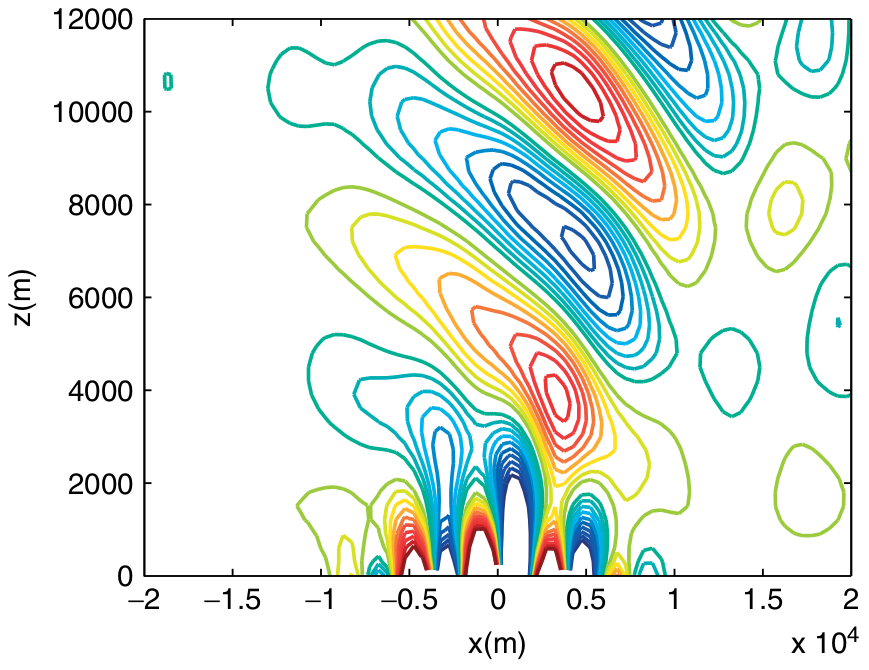
\includegraphics[height=2in]{img/melvin-7a.png}} \\
	\subcaptionbox{SLEVE \label{fig:gw:w:sleve}}[0.48\textwidth]{\includegraphics[height=2.6in,angle=270]{data/gravityWaves-sleve-schaerExp-h/18000/w.eps}}
	\hfill
	\subcaptionbox{SLEVE \label{fig:gw:thetaDiff:sleve}}[0.48\textwidth]{\includegraphics[height=2.6in,angle=270]{data/gravityWaves-sleve-schaerExp-h/18000/thetaDiff.eps}} \\
	\subcaptionbox{SnapCol \label{fig:gw:w:snapCol}}[0.48\textwidth]{\includegraphics[height=2.6in,angle=270]{data/gravityWaves-snapCol-schaerExp-h/18000/w.eps}}
	\hfill
	\subcaptionbox{SnapCol \label{fig:gw:thetaDiff:snapCol}}[0.48\textwidth]{\includegraphics[height=2.6in,angle=270]{data/gravityWaves-snapCol-schaerExp-h/18000/thetaDiff.eps} \TODO{include legend}}
	\caption{\TODO{w contours, every \SI{5e-2}{\meter\per\second}.  $t = \SI{18000}{\second}$ Compared with fig 7a from \textcite{melvin2010}.}}
	\label{fig:gw:w}
\end{figure}

Comparing vertical velocity contours between BTF and SLEVE show few visible differences (figures~\ref{fig:gw:w:btf}, \subcaptionref{fig:gw:w:sleve}).  Since the same model was used, these results match those from \textcite{weller-shahrokhi2014}.  Vertical velocities on the SnapCol grid are similar to the terrain following results (figure~\ref{fig:gw:w:snapCol}).  All three results are in agreement with a semi-implicit, semi-Lagrangian simulation from \textcite{melvin2010} (see figure~\ref{fig:gw:w:melvin}).

\begin{figure}
	\captionsetup[subfigure]{position=b}
	\centering
	\subcaptionbox{SLEVE \label{fig:gw:thetaDiffZoom:sleve}}[\textwidth]{\includegraphics[width=1.6in,angle=270]{data/gravityWaves-sleve-schaerExp-h/18000/nonlinearMomentumZoom.eps}} \\
	\subcaptionbox{SnapCol \label{fig:gw:thetaDiffZoom:snapCol}}[\textwidth]{\includegraphics[width=1.6in,angle=270]{data/gravityWaves-snapCol-schaerExp-h/18000/nonlinearMomentumZoom.eps}}
	\caption{\TODO{Theta anomalies (zoomed in)}}
	\label{fig:gw:thetaDiffZoom}
\end{figure}

Theta anomalies are similar on all grids, having a similar shape to vertical velocity contours, but phase shifted by \ang{180} (SLEVE grid figure~\ref{fig:gw:thetaDiff:sleve}, SnapCol grid figure~\ref{fig:gw:thetaDiff:snapCol}, BTF grid not shown). 
Examining more closely the potential temperature anomaly on the SnapCol grid, in the lee of the mountain the bottommost layer is anomalously warm and the layer above it is anomalously cold (figure~\ref{fig:gw:thetaDiffZoom:snapCol}).  Potential temperature increases with height because the simulated atmosphere is stable, so these anomalies serve to reduce the stability near the ground.  The anomalies are not sufficiently large to destabilise the atmosphere, however.   Therefore, vertical motion is not expected, and was not observed, near the ground on the lee side.   Whilst turbulent motion does cause thermal mixing in the real atmosphere, there is no viscosity in the model equations, so the thermal anomalies should not be present.  The feature is not present on the SLEVE grid (figure~\ref{fig:gw:thetaDiffZoom:sleve}) or BTF grid (not shown).

\TODO{Train of thought leading to hypothesis that computational mode in Lorentz staggering is excited by advection errors.}

\begin{figure}
	\captionsetup[subfigure]{position=b}
	\centering
	\subcaptionbox{SLEVE}[\textwidth]{\includegraphics[width=1.6in,angle=270]{data/gravityWaves-sleve-schaerExp-h/18000/UfZoom.eps}} \\
	\subcaptionbox{SnapCol}[\textwidth]{\TODO{}} \\
%
	\caption{\TODO{SLEVE and SnapCol flows}}
	\label{fig:gw:flow}
\end{figure}

\begin{figure}
	\centering
	\input{gravityWaves-schaerExp-h-exnerTheta-plot}
	\caption{\TODO{exner/theta sample line at $x = \SI{50}{\kilo\meter}$}}
	\label{fig:gw:exner-theta}
\end{figure}

\TODO{we tried a bunch of other things: double height mountains, halving $\Delta z$, and managed to get mixing to appear in BTF, too.  we also looked at nonlinear momentum term although I'm not 100\% sure what that told us.  also looked at energy changes but, unlike resting atmosphere, we might expect energy loss here... due to the sponge layer?  nevertheless, energy loss is greater on snapCol grid compared to BTF/SLEVE grids}

\begin{figure}
	\captionsetup[subfigure]{position=b}
	\centering
	\subcaptionbox{Maximum Courant number \label{fig:gw:courant:max}}[0.49\textwidth]{\input{gravityWaves-courant-max-plot}}
	\hfill
	\subcaptionbox{Mean Courant number \label{fig:gw:courant:mean}}[0.49\textwidth]{\input{gravityWaves-courant-mean-plot}}
	%
	\caption{Courant numbers on BTF, SLEVE and SnapCol grids for the gravity waves test.}
	\label{fig:gw:courant}
\end{figure}

No evidence of the `small cell' problem associated with cut cell grids, discussed in section~\ref{sec:theory:shaving},  has been found on the SnapCol grid.  At each timestep, the maximum and mean Courant number for all cells in the grid was calculated.  Whilst initially larger on the SnapCol grid, the maximum Courant number eventually converges for all three grids (figure~\ref{fig:gw:courant:max}).  The mean Courant number is similar across all grids throughout the simulation (figure~\ref{fig:gw:courant:mean}).  \TODO{the mean and max do increase slowly over time.  this is more obvious in longer simulations.  this seems bad.  worth mentioning?}

\begin{figure}
	\centering
	\documentclass[tikz]{standalone}
\usepackage{bm}
\usetikzlibrary{arrows}
\newcommand{\vect}{\bm}
\newcommand{\del}{\nabla}

\newcommand{\trans}[1]{{#1^\star}}
\newcommand{\surface}{h}
\newcommand{\shellcmd}[1]{\texttt{#1}}
\newcommand{\diffusioncoeff}{\mathcal{D}}
\newcommand{\exner}{\Pi}
\newcommand{\courant}{\mathrm{Co}}

\begin{document}
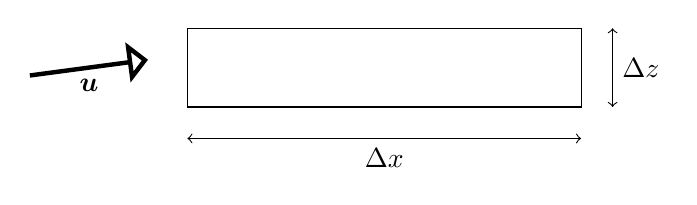
\begin{tikzpicture}[
  cpnt/.style={fill=gray},
  arr/.style={thick, ->},
]
\draw (5,1) rectangle (10,2);

\draw [<->] (5,0.6) -- (10,0.6) node [midway, below] {$\Delta x$};
\draw [<->] (10.4,1) -- (10.4,2) node [midway, right] {$\Delta z$};

\draw [->, >=open triangle 90, ultra thick] (3,1.4) -- (4.5,1.6) node [midway, below] {$\vect{u}$};
\end{tikzpicture}
\end{document}

	\caption{Nearly-horizontal flow through a thin, rectangular cell in the $x-z$ plane.  Because the vertical velocity component is small, the cell height $\Delta z$ has a negligible effect on the two-dimensional Courant number.}
	\label{fig:gw:small-cell}
\end{figure}

This can be explained by considering flow through a two-dimensional, rectangular cell in the $x-z$ plane in which $\Delta x$ is several times larger than $\Delta z$ (figure~\ref{fig:gw:small-cell}).  Using equation~\ref{eqn:method:courant} and assuming a uniform flow $\vect{u} = ( u, 0, w )^\intercal$, the Courant number is
\begin{align}
	\courant &= \frac{\Delta t}{\Delta x \Delta z} \left( u \Delta z + w \Delta x \right)
%
	\intertext{When the flow is almost horizontal, $u \gg w$, so}
%
	\courant &\approx \frac{u \Delta t}{\Delta x}
\end{align}
That is, the two-dimensional Courant number reduces to the one-dimensional Courant number.  Hence, the cell height $\Delta z$ has little effect on the CFL criterion.

In the gravity waves test, vertical motion is induced by the terrain and, for the shallow gradients used in this test, horizontal velocities dominate (see figure~\ref{fig:gw:flow}).

\hrule

\hrule
\TODO{these are just notes...}

\begin{itemize}
\item Vertical mixing at ground in lee of orography seen in results for snapCol and snap meshes.  This occurs in the lowest two rows of the mesh: lower layer $\theta$ is warmer, next layer above is cooler.  Feature is visible after t=3600s (Figure~\ref{fig:gw:mixing-3600s}), becomes more pronounced by t=18000s (Figure~\ref{fig:gw:mixing-18000s}).
\end{itemize}

\subsection{Investigation of vertical mixing}
Initially suspected mixing was due to computation mode of Lorenz vertical staggering but now it seems not (or maybe it does! we're not quite sure!)
\begin{itemize}
	\item plot UfDiff as a vector field doesn't seem to show any velocity anomalies in BTF or snalCol (Figure~\ref{fig:gw:ufdiff})
	\item plot of $\theta$ field shows that mixing is not strong enough to overcome stratification (Figure~\ref{fig:gw:theta})
	\item doubling mountain height causes mixing to appear in BTF case, and increases to three rows of mixing in SnapCol (Figure~\ref{fig:gw:double-height})
	\item halving $\Delta z$ also causes BTF mixing but less severe, also three rows of mixing in SnapCol (not shown)
	\item the results for dp/dx show mixing in BTF, and increased mixing in SnapCol (not shown)
\end{itemize}


By isolating the nonlinear advection term in the momentum equations ($\del \rho \vect{u} \vect{u}$) we can see the different in flows between BTF and SnapCol meshes (Figure~\ref{fig:gw:nonlinear-advection}).  Looking at $U_f$ we can see larger velocities in small cells near mountain peaks, but otherwise flow fields are qualitatively in good agreement.

Noticing that $U_f$ follows the BTF mesh but does not follow the SnapCol mesh, we suspect that the thermal mixing may be caused by numerical diffusion (as we same with horizontal tracer advection).  This time, however, the flow is not horizontal, so it is SnapCol that has more diffusion.

\subsection{Courant number}

\begin{itemize}
	\item Mean Courant numbers for cut-cell meshes and SLEVE are lower than BTF.  This could be because cells are relatively smaller aloft.
\end{itemize}

\subsection{Energy}
\begin{itemize}
	\item Cut cell meshes are worse than TF meshes.  Snap loses internal energy much quicker than other meshes; i.e. it gets colder. (Figure~\ref{fig:gw:energy})
\end{itemize}

\begin{figure}
	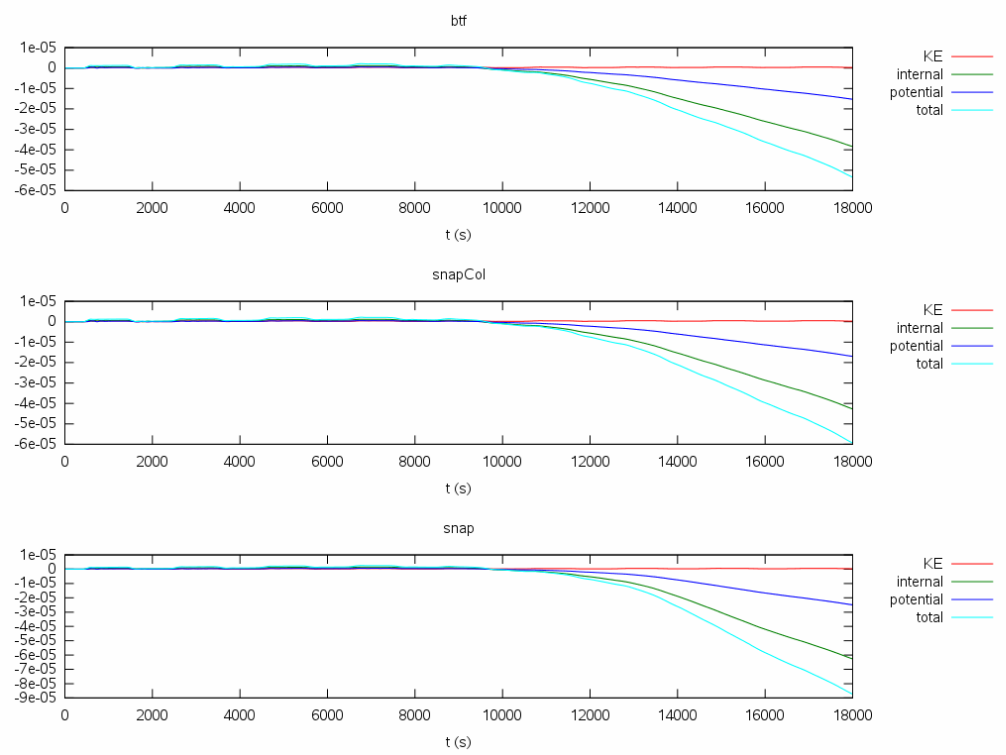
\includegraphics[width=\textwidth]{interim-results/gravityWavesEnergy.png}
	\caption{Energy changes}
	\label{fig:gw:energy}
\end{figure}

Looking at max Courant number for SLEVE, and energy loss graphs for all meshes, we see a change of behaviour at t=10000s (about 2.8 hours).  This might be related to gravity waves reflecting off the inlet or outlet boundary.  Changing the wind speed would let us investigate further.
